\chapter{Detalles de Implementación y Experimentos}\label{chapter:implementation}

La implementación está hecha en \textbf{Python 3} \cite{python3} haciendo uso de las blibliotecas \textbf{Sympy} \cite{10.7717/peerj-cs.103}, 
\textbf{Scipy} \cite{2020SciPy-NMeth} y \textbf{PyWavelets} \cite{Lee2019}. Todos los experimentos se 
realizaron en \textbf{Jupyter Notebooks} \cite{Kluyver2016jupyter} y al igual que la DST-II están disponibles en el repositorio de
GitHub.

\section{Solución numérica del sistema de ecuaciones no lineales}

Como primer paso para la construcción de la \textit{shapelet} es necesario resolver un sistema de ecuaciones
no lineales. Dado que el número de ecuaciones y variables, así como de los coefecientes varía en dependencia
del patrón que se requiere reconocer, es necesario generar dinámicamente el sistema de ecuaciones. Con la ayuda
de Sympy \cite{10.7717/peerj-cs.103} esto se logra de forma fácil y sencilla. Luego, para encontrar una solución 
se analizaron varios métodos numéricos de optimización.

Los métodos analizados fueron \textit{hybr}, \textit{lm}, \textit{broyden1}, \textit{broyden2} y \textit{krylov}.
El primero es una modificación del método de Powell y el segundo es el método de mínimos cuadrados Levenberg-Marquardt.
Para ambos casos se usó la implementación de MINPACK \cite{osti_6997568} a través de \textbf{scipy.optimize.root}. Los restantes
algoritmos son todos métodos de Newton inexactos, que usan \textit{backtracking}  y búsquedas completas lineales. Cada
método corresponde a una aproximación particular del jacobiano

\subsection{Diseño de los experimentos}

\begin{figure} 
	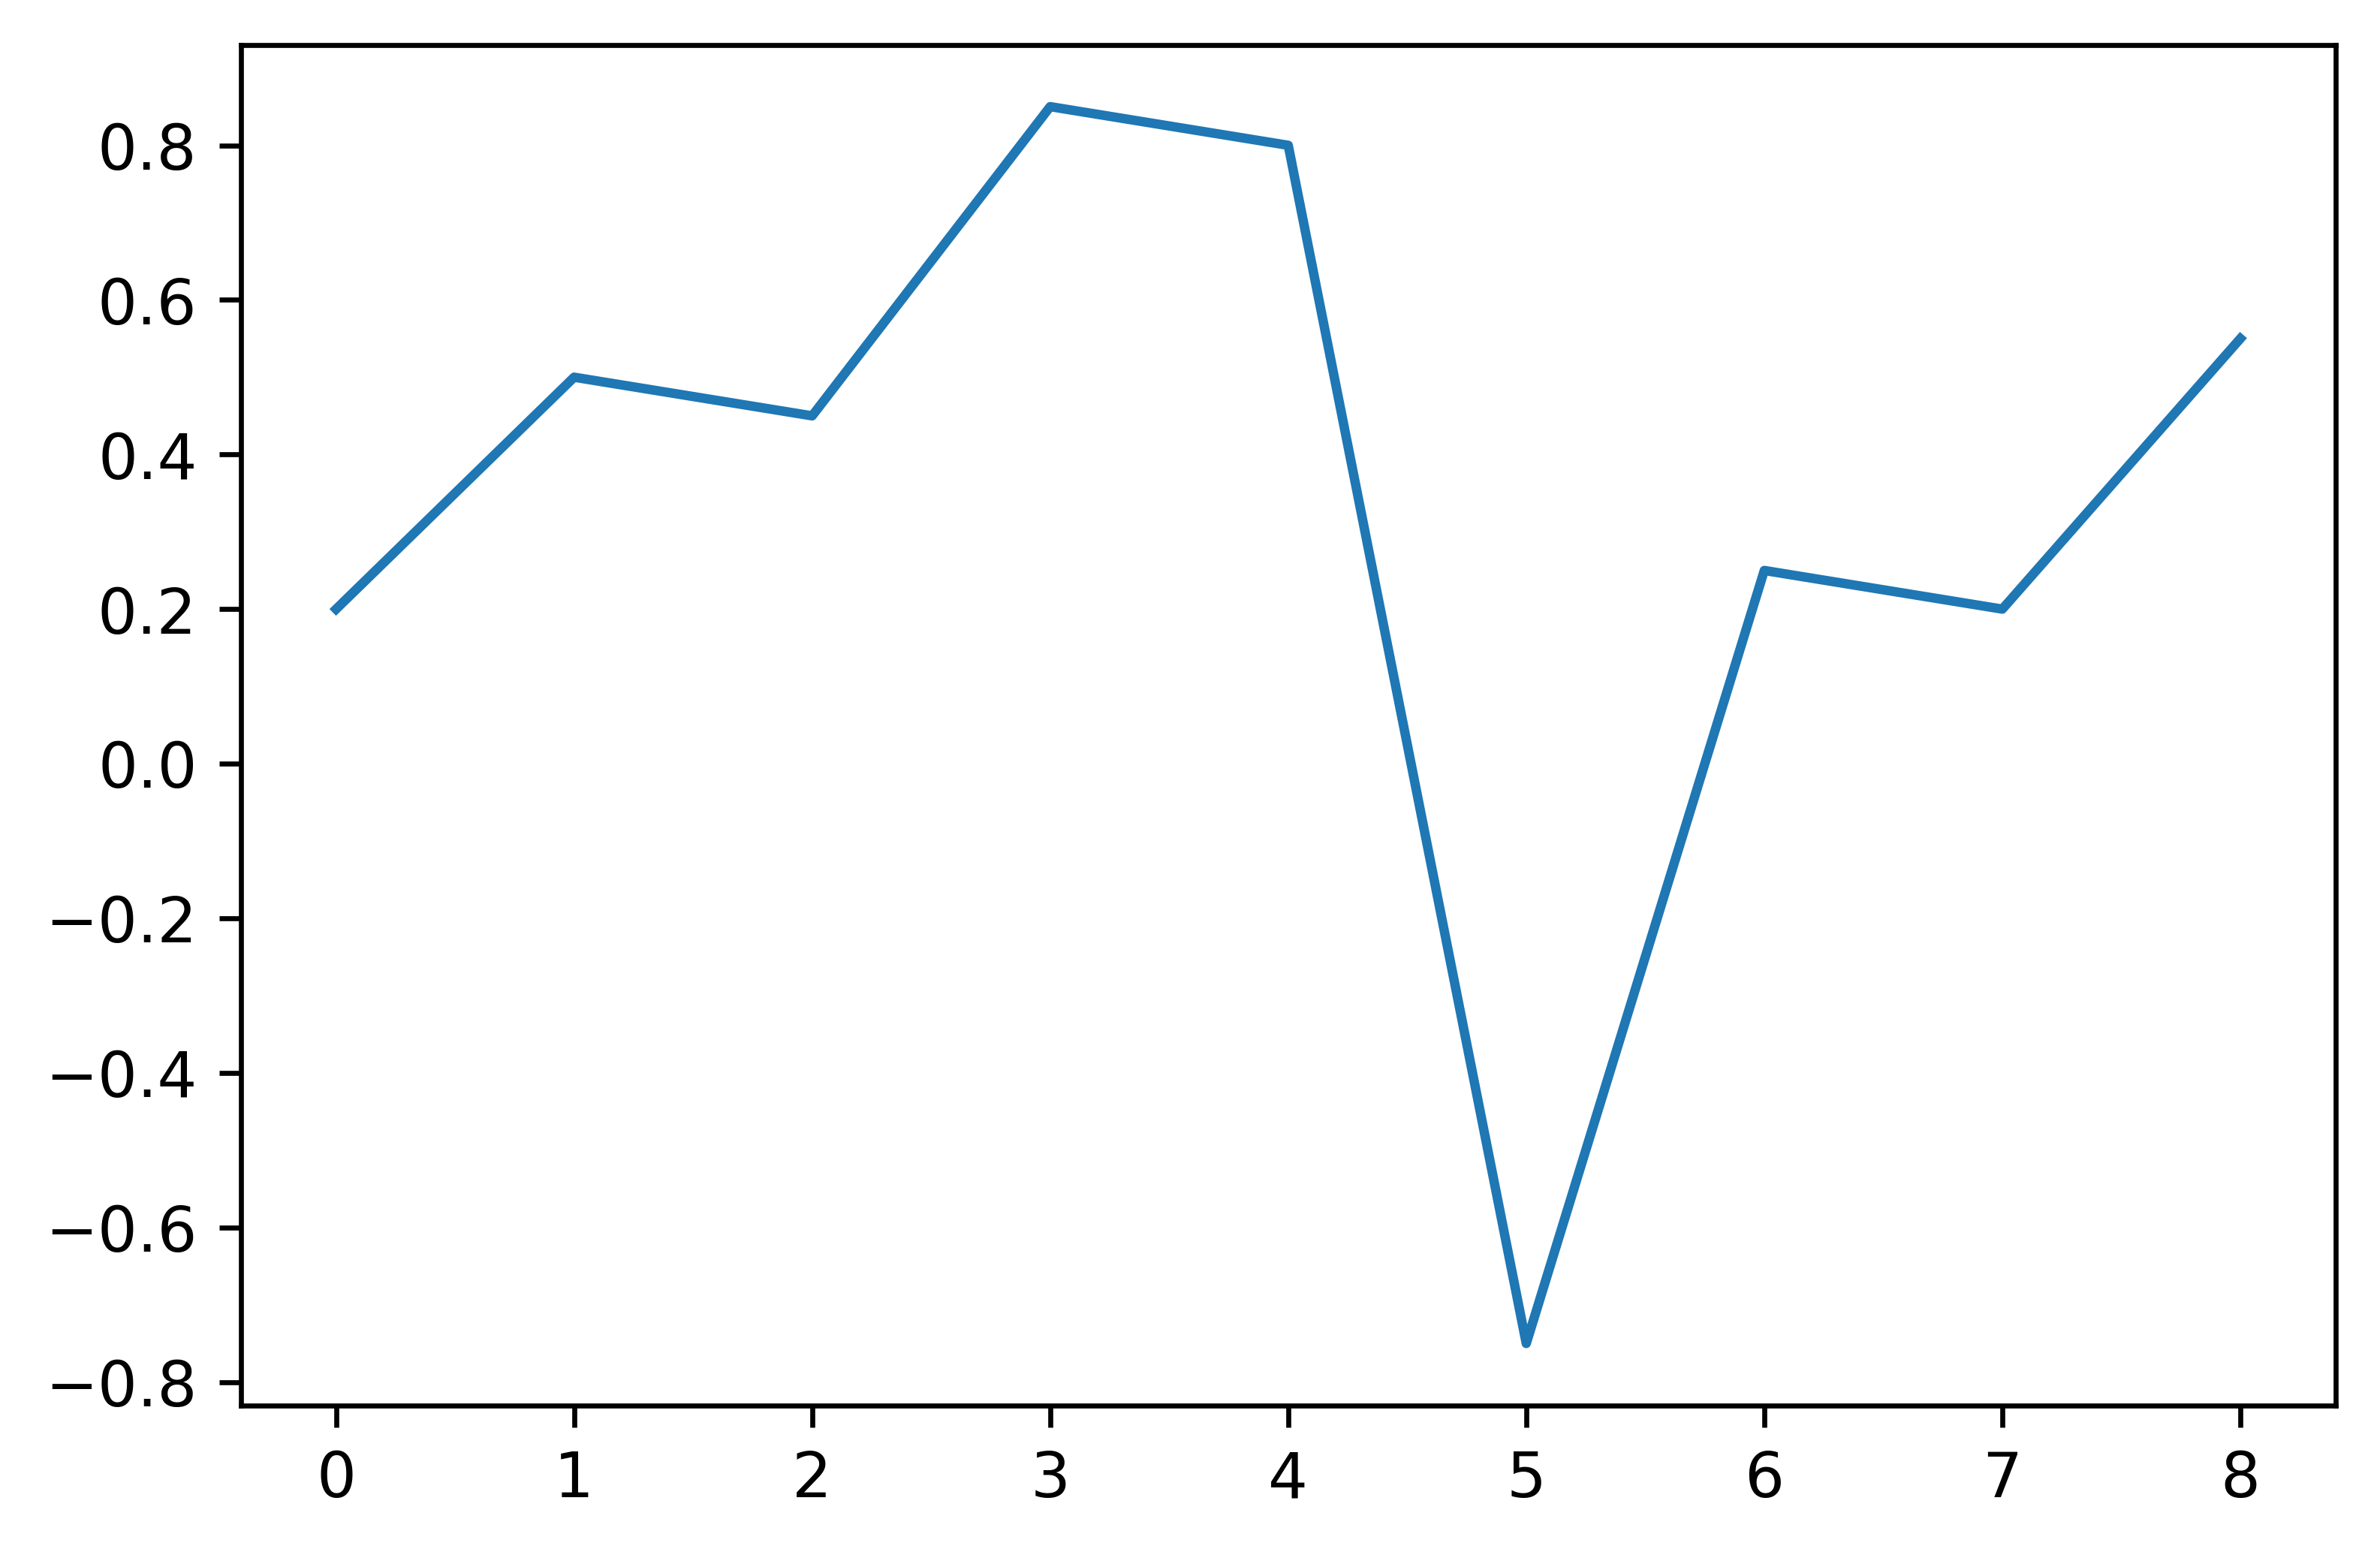
\includegraphics{Graphics/guido20118-pattern.png}
	\caption{Patrón usado en \cite{Guido2018} con valores [0.20, 0.50, 0.45, 0.85, 0.80, -0.75, 0.25, 0.20, 0.55]}\label{fig:Guido2018-pattern}
\end{figure}

Para la selección de los métodos primeramente se utilizó el patrón \ref{fig:Guido2018-pattern} y se compararon los
resultados entre los distintos métodos numéricos y la solución mostrada en \cite{Guido2018}.

\begin{table}[h!]
	\centering
	\begin{tabular}{|c|c|c|} \toprule
		Método &  Convergencia & Error \\ \midrule
		hybr   &  Si         & 5.13527681450854E-14 \\
		lm   &  Si           & 1.32847208829431E-16 \\ 
		broyden1   &  Si     & 0.00000288748001856531 \\ 
		broyden2   &  No     & 1.05694754160886E+20 \\ 
		anderson   &  Si     & 0.00000147755764075454 \\
		linearmixing   &  No  & 9.97441058654864E+16 \\
		diagbroyden   &  No  & 9.42301917618925E+46 \\
		krylov   &  No       & 1.00000000000000  \\ \bottomrule
	\end{tabular}
	\caption{Tabla del error de las soluciones de los distintos algoritmos para el patrón \ref{fig:Guido2018-pattern}}\label{table:error-pattern-guido}
\end{table}
 
